\documentclass{article}
\usepackage[toc,page]{appendix}
\newcommand{\nocontentsline}[3]{}
\newcommand{\tocless}[2]{\bgroup\let\addcontentsline=\nocontentsline#1{#2}\egroup}

%%%% Bibliography %%%%%
\usepackage[backend=biber, style = numeric, url = false, maxcitenames=1,  citestyle=numeric-comp]{biblatex}
\renewcommand{\citet}[1]{\citeauthor{#1} (\citeyear{#1})}

\addbibresource{Bibliography.bib}
%%%% Bibliography %%%%%

\usepackage[pagestyles]{titlesec}
\usepackage[x11names]{xcolor}
\definecolor{light_yellow}{RGB}{255, 255, 153}
\definecolor{occer}{RGB}{176, 150, 20}
\definecolor{ILIAS_grey}{RGB}{240,240,240}
\definecolor{anthracite}{RGB}{100, 100, 100}
\definecolor{grayish}{RGB}{180, 180, 180}
\definecolor{graylight}{RGB}{220, 220, 220}
\definecolor{unibe}{RGB}{194,1,45}
\usepackage{amsfonts}
\usepackage{amsmath}
\usepackage{textcomp}
\usepackage{enumerate}
\usepackage{tikz}
\usepackage{bibentry}
\usepackage{enumitem}
\usepackage[a4paper]{geometry}
\usepackage{minitoc}
\usepackage{capt-of}
\usepackage{caption}
\setcounter{secnumdepth}{5}
\usepackage{lipsum}
\usepackage{calc}
\usepackage[T1]{fontenc}
\usepackage{etoolbox}
\usepackage[absolute]{textpos}
\usepackage{chngcntr}
\usepackage{ifthen}
\usepackage{titling}
\usepackage{authblk}
\usepackage{booktabs}

\providetoggle{footrule}
\providetoggle{fancytitles}
\providetoggle{headrule}
\let\counterwithout\relax
\let\counterwithin\relax

% --- user editable parameters --- 
\settoggle{footrule}{false} %include footer rule (True) or not (False)
\settoggle{headrule}{false} %include footer rule (True) or not (False)
\settoggle{fancytitles}{false} %use fancy paragraph titles
%\usepackage{showframe}
% --- --- --- --- --- --- --- ---

% --- User editable numbering scheme ---
\counterwithin*{figure}{section}
\counterwithin*{table}{section}
\counterwithin{subsection}{section}
% --- Labelling scheme ---
\renewcommand{\thesection}{\arabic{section}}
\renewcommand{\thesubsection}{\thesection .\arabic{subsection}}
\renewcommand\thesubsubsection{\thesubsection.\arabic{subsubsection}}
\captionsetup[table]{labelfont={color=\titleschemecolor, bf},labelsep=quad, textfont=small }
\captionsetup[figure]{labelfont={color=\titleschemecolor, bf},labelsep= quad, textfont=small }
% --- --- --- --- --- --- --- --- --- ---

\setlength{\TPHorizModule}{30mm}
\setlength{\TPVertModule}{\TPHorizModule}
\textblockorigin{10mm}{10mm} % start everything near the top-left corner
\setlength{\parindent}{0pt}
\dimendef\prevdepth=0
\counterwithin*{figure}{section}
\counterwithin*{table}{section}
\counterwithin{subsection}{section}

\iftoggle{footrule}{
\newcommand{\btm}{1.8cm} 
\newcommand{\fskp}{0.6cm}
\newcommand{\flpa}{0.42}
\newcommand{\flpb}{9.44}
\newcommand{\frpa}{4.1}
\newcommand{\frpb}{\flpb}
}{
\newcommand{\btm}{1.8cm} 
\newcommand{\fskp}{0.22cm}
\newcommand{\flpa}{0.33}
\newcommand{\flpb}{9.44}
\newcommand{\frpa}{4.2}
\newcommand{\frpb}{\flpb}
}

\iftoggle{headrule}{\newcommand{\tp}{25pt}}{\newcommand{\tp}{18pt}}

%abstract formatting
\renewenvironment{abstract}{%
\vspace{-10pt}
\begin{minipage}{0.47\textwidth}
\textcolor{\titleschemecolor}{ABSTRACT}}
{\vspace{5pt}\newline\color{\authorcolor} \titlerule
\end{minipage}}

\newpagestyle{TLS_report_2}{
\newgeometry{a4paper, left = 2cm, right = 2cm, bottom = \btm, top = 0cm, twoside, twocolumn, includehead, includefoot, footskip = \fskp}
\ifthenelse{\equal{\docfont}{helvetica}}{\renewcommand*{\familydefault}{\sfdefault}}{}
\setlength{\columnsep}{0.9cm}
\setlength\headsep{\tp} %used to be 80
\setlength{\headheight}{1.25cm}
\setlength{\voffset}{-1.1in}
\setlength{\topmargin}{0pt}
\newcommand{\hbh}{50}%headbox height
\newcommand{\hbl}{25}%headbox length
\newcommand{\hrl}{0.99\linewidth - \hbl - \hbl}

\renewcommand\Affilfont{\itshape\small}

%Title Formatting
\pretitle{%\vspace{-10pt} 
\begin{minipage}{\linewidth}
\flushleft \bfseries \fontsize{155}{199}\Large\selectfont \textcolor{\titleschemecolor} } 
\posttitle{\vspace{10pt}\end{minipage}
}
\preauthor{\flushleft \large \textcolor{\authorcolor}}
\postauthor{\newline \vspace{10pt}}
\predate{\color{\authorcolor} \titlerule \newline \flushright \vspace{-30pt}}


\iftoggle{fancytitles}{
\titleformat{\section}{\fontsize{14}\large\bfseries\textcolor{\titleschemecolor}}{}{0pt}{\textcolor{\titleschemecolor}{\thesection} \hspace{5pt} \bfseries}%[][\vspace{6pt} {\titlerule[0.9pt]}]


\titleformat{\subsection}{\fontsize{13}\linespread\large\bfseries}{}{0pt}{\textcolor{\titleschemecolor}{\thesubsection} \hspace{5pt} }[\vspace{6pt} {\titlerule[0.9pt]} \vspace{3pt}]
\titlespacing*{\subsection}{0pt}{25pt}{10pt}

\titleformat{\subsubsection}{\fontsize{11}\large\bfseries}{}{0pt}{{\thesubsubsection} \hspace{5pt} \bfseries}[\vspace{-1pt}]
}{
\titleformat{\section}{\fontsize{14}\large\bfseries\textcolor{\titleschemecolor}}{}{0pt}{\textcolor{\titleschemecolor}{\thesection} \hspace{3pt} \bfseries}%[][\vspace{6pt} {\titlerule[0.9pt]}]

\titleformat{\subsection}{\fontsize{13}\linespread\large\bfseries}{}{0pt}{%\textcolor{\titleschemecolor}{\thesubsection} \hspace{5pt} 
	}[]%\vspace{6pt} {\titlerule[0.9pt]} \vspace{3pt}]
\titlespacing*{\subsection}{0pt}{25pt}{10pt}

\titleformat{\subsubsection}{\fontsize{11}\linespread\large\bfseries}{}{0pt}{
	%{\thesubsubsection} \hspace{5pt} \bfseries
	}[\vspace{-1pt}]

}

\sethead[
\makebox(\hbh, \hbl)[b]{
\colorbox{\boxcolor}{\makebox(\hbh, \hbl)[b]{\Large \bfseries  \textcolor{\boxtextcolor} \evenboxcontent \vspace{5pt} }}}
\hspace{3pt}
\iftoggle{headrule}{
\color{\rulecolor}\titlerule
}{}
][][
\begin{textblock}{2}(4.1,0.625)
\begin{flushright}
	\large \bfseries \textcolor{\titleschemecolor}{ \thesection \hspace{4pt} $|$ \hspace{1.5pt} \sectiontitle }
\end{flushright}
\end{textblock}
]
{
\begin{textblock}{5.801}(0.42,0.9255)
\iftoggle{headrule}{ %%%%%%%%%%%
	\color{\rulecolor}\titlerule 
}{}
\end{textblock}
\begin{textblock}{2}(0.42,0.74)
\large \bfseries \textcolor{\titleschemecolor}\doctype
\end{textblock}


}{}{
\begin{textblock}{2}(5.6,0.637)
\makebox(\hbh, \hbl)[b]{
\colorbox{\boxcolor}{\makebox(\hbh, \hbl)[b]{\Large \bfseries  \textcolor{\boxtextcolor} \oddboxcontent \vspace{5pt} }}}
\end{textblock}
}

\setfoot[
\iftoggle{footrule}{\color{\secondaryrulecolor}\titlerule}{}
\begin{textblock}{2}(\flpa,\flpb)
\begin{flushleft}
	\textcolor{\secondaryschemecolor}{ \footleft}
\end{flushleft}
\end{textblock}
][][
\begin{textblock}{2}(\frpa,\frpb)
\begin{flushright}
	\textcolor{\secondaryschemecolor}{ \footright}
\end{flushright}
\end{textblock}
]{
\iftoggle{footrule}{\color{\secondaryrulecolor}\titlerule}{}
\begin{textblock}{2}(\flpa,\flpb)
\begin{flushleft}
	\textcolor{\secondaryschemecolor}{ \footleft}
\end{flushleft}
\end{textblock}
}{}{
\begin{textblock}{2}(\frpa,\frpb)
\begin{flushright}
	\textcolor{\secondaryschemecolor}{ \footright}
\end{flushright}
\end{textblock}
}

}




%customise color scheme
\newcommand{\rulecolor}{grayish}
\newcommand{\secondaryrulecolor}{\rulecolor}

\newcommand{\boxcolor}{grayish}
\newcommand{\boxtextcolor}{white}

\newcommand{\titleschemecolor}{unibe}
\newcommand{\secondaryschemecolor}{\authortitlecolor}

\newcommand{\toccolor}{black}
\newcommand{\authorcolor}{anthracite}

\newcommand{\docfont}{helvetica} %helvetica or times
\newcommand{\headfont}{helvetica} %helvetica or times
%-----------------------

%define what kind of Report is being written in the peripheries
\newcommand{\doctype}{BC I Practical \hspace{6pt} $\boldsymbol{|}$ \hspace{6pt} Report} %odd pages header
\newcommand{\evenboxcontent}{\vspace{-4.5pt} 
\includegraphics[width = 20pt]{Resources/ub_w}} % content of the box on even pages
\newcommand{\oddboxcontent}{\evenboxcontent} % content of the box on odd pages
\newcommand{\footright}{\thepage} %footer right
\newcommand{\footleft}{\large Communications in Biochemistry} %footer left

%Document Information and Title
\title{Identification of Human Genetic Locus from Unknown Meat Sample by Restriction Fragment Length Polymorphism}
\author[1]{Noah H. Kleinschmidt} %to add affiliation, place the respective sign (number) in [] in front of author, then add \affil with the number and institution.
\affil[1]{Universit\"at Bern}
\date{04.04.2020}

\pagestyle{TLS_report_2}
\begin{document}

\pagenumbering{arabic}
\setcounter{page}{1} 
\maketitle
\thispagestyle{TLS_report_2}

%\begin{abstract}
%	Catalase is an enzyme, charged with protecting cells from oxidative damage by reactive oxygen species hydrogen peroxide. It has been found in all studied aerobic organisms and neutralises reactive $H_2O_2$ into water and molecular oxygen. In this experiment kinetic properties of catalase obtained from potato extract were studied. To that end, oxygenic activity, associated with catalase-mediated $H_2O_2$ decomposition, was monitored. As expected from enzymes that follow Michaelis Menten kinetics, both enzyme and substrate concentrations were found to positively affect catalatic activity. The pH Optimum could be traced around pH 8, which is in accordance with currently published data. Hydroxylamine, an inhibitor of catalase, could be shown to likely affect catalase by a competitive mechanism. \citet{PCRorig}.
%\end{abstract}

%include all Sections that are to be part here...	
%Everything inside the Introduction Section (no Chapters)
\begin{multicols}{3}

\section{Introduction}

%Everything inside the Introduction Section (no Chapters)
\section{Introduction}

\section{Effect of population heterogeneity in disease dynamics}
\subsection{A project for Computational Epidemiology (Course: 467294-HS2021)}

This project models the effect of two subgroups within a population that are either "normally" susceptible (default average person) or "highly" susceptible to a disease (perhaps due to immuno-suppression because of other medical issues). As such, "normally" susceptibles ($S_n$) and "highly" susceptibles ($S_h$) are assumed to have also different rates of recovery.

## SIR Model 
---
\subsection{Susceptible Population $S$}
This project assumes the total population $S$ consists of two groups as per:

%\begin{equation}
%\begin{split}
%	
%S & = S_n + S_h = \alpha_n  \cdot S + \alpha_h \cdot S \\
%  & = \alpha_n  \cdot S + (1-\alpha_n)\cdot S
%\end{split}
%
%\end{equation}

where $\alpha_i$ are the percentages of each group within the population. 

\subsection{Infectious Population $I$}
As both $S_n$ and $S_h$ are assumed to have different susceptibilities, they are assigned two different rates of infection: $\beta_n$ and $\beta_h$, where we assume for simplicity sake that $\beta_h = k\cdot\beta_n$ for some $k > 1 \in \R$. 




\subsection{Removed Population $R$}
Removed (recovered or deceased) cannot be infected nor infect others. Both $S_n$ and $S_h$ have a recovery rate that assigns them to this population. Yet, we assume that the two groups have different rates of recovery $\gamma_n$ and $\gamma_h$. We again assume for simplicity sake that $\gamma_h = j\cdot\gamma_n$ for some $j < 1 \in \R$. The total rate at which $R$ increases is hence $\gamma_n + \gamma_h = \gamma_n + j\gamma_n = (1+j)\gamma_n$.
%
%\subsection{Preliminary SIR System of Equations}
%As both infection rate and recovery rate are ultimately just determined by the rate for the "normally" susceptibles we abbreviate $\beta_n \equiv \beta$ and $\gamma_n \equiv \gamma$.
%
%The implemented system of differential equations is hence: 
%
%$$
%\begin{align}
%
%\frac{dS(t)}{dt} = {}&  [\ -\beta \cdot S_n(t) - k\beta \cdot S_h(t) \ ] \cdot I(t) \\
%\frac{dI(t)}{dt} = {}&  [\ \beta \cdot S_n(t) + k\beta \cdot S_h(t) \ ] \cdot I(t) - (1 + j)\gamma\cdot I(t) \\
%\frac{dR(t)}{dt} = {}&  (1 + j)\gamma\cdot I(t)
%
%\end{align}
%$$
%
%
%This system we can simplify slightly by aggregating the infectous transition for $S_n$ and $S_h$ as follows, thus modifying $\frac{dS(t)}{dt}$ and $\frac{dI(t)}{dt}$:
%
%$$
%\begin{align}
%
%\frac{dS(t)}{dt} = {}&  -\beta(\alpha_n  + k (1 -\alpha_n)) \cdot S(t)\cdot I(t) \\
%\frac{dI(t)}{dt} = {}&  \beta(\alpha_n  + k (1 -\alpha_n)) \cdot S(t)\cdot I(t) - (1 + j)\gamma\cdot I(t) \\
%
%\end{align}
%$$
%

\subsection{Relapsation of susceptibles}
In our preliminary model we assume two groups within the population, the "normal" and "highly" susceptibles. We further assume that, although they both have different rates of infection and recovery, they ultimately endure the same course of disease, going from susceptible, to infectous, and ultimately to removed. However, what if this assumption were not true, and a small part of the population were to relapse into the susceptible population $S$ after having endured the infectuous stage? 

This could be the case for immuno-suppressed inviduals who did survive the disease due to medical care but were unable to fully develop their own immune response. Alternatively, normally susceptibles may have endured a more severe course of disease that weakened their immune system, thus pushing them to the highly susceptibles after having left the infectuous stage. 

\subsubsection{Relapsation Rate $\delta$}
Both of the above scenarious are somewhat complex, and shall be addressed in a simplified manner by introducing a relapsation rate $\delta_i$ for both normally and highly susceptibles. $\delta_i$ allows removed people to leave $R$ to re-enter $S$ as part of the highly susceptibles $S_h$. Thereby, $\frac{dS(t)}{dt}$ will be modified to receive an additive term from $R$, and $\frac{dR(t)}{dt}$ will receive a corresponding subtractive term. As we assume normal and highly susceptibles will have different rates of relapsation, we will use our default asumption of $\delta_h = h \cdot \delta_n$ for some $h \in \R$ (no restriction to bigger or smaller 1).

\subsection{Relapsation SIR System of Equations}
We retain $\beta_n \equiv \beta$ and $\gamma_n \equiv \gamma$, and abbreviate $\delta_n \equiv \delta$.
The implemented system of differential equations is hence: 

\begin{align*}

$\frac{dS(t)}{dt} &=  -\beta(\alpha_n  + k (1 -\alpha_n)) \cdot S(t) \cdot I(t) + \delta(1 + h) \cdot R(t)$ \\

$\frac{dI(t)}{dt} &=  \beta(\alpha_n  + k (1 -\alpha_n)) \cdot S(t) \cdot I(t) - (1 + j)\gamma\cdot I(t)$ \\

$\frac{dR(t)}{dt} &=  (1 + j)\gamma\cdot I(t) - \delta(1 + h) \cdot R(t)$


\end{align*}


\subsection{Lethality versus Recovery}
The model outlined so far has treated recovered and deceased as equivalent. However, considering the assumtion above of some more susceptible groups that may also have a higher relapsation rate, the concept of lethality should be taken into consideration as well. Immuno-suppressed individuals may very likely have a higher risk of actually dying rather than recovering. This would impact the subtractive term of $\frac{dI(t)}{dt}$ (additive in $\frac{dR(t)}{dt}$), as only a sub-group of removed may be able to relapse, namely the ones who survived. To address this we modify the model to split the current $R$ into two groups $R'$ (recovered, who may relapse) and $D$ (deceased, who may not relapse). Admitedly, this does leave the \textit{SIR} model for an "\textit{SIRD}" model (not sure about terminlolgy?), but seems to mimic disease dynamics better under the given assumptive parameters. 

\subsubsection{Death rate $\theta$}
To split the current $R$ (removed) we adjust the rate of transition from $I$ to $R$ for the two new subgroups of $R$, we introduce a lethality rate $\theta$ as a percentage of people who transition to $R$ due to death rather than recovery. $\theta$ modifies the current recovery rate $\gamma$ to a new recovery rate $\gamma' = (1 - \theta)\gamma$. 
We again assume that highly susceptibles have a different death rate than normally susceptibles: $\theta_h = q \cdot \theta_n$ for some $q > 1 \in \R$. 


The new transition from $I$ to $R'$ or $D$ is hence: 

$$
\begin{aligned}
\frac{dI(t)}{dt} = {}&  \beta(\alpha_n  + k (1 -\alpha_n)) \cdot S(t) \cdot I(t) - (1 + j)\gamma'\cdot I(t) - (1 + q)\theta\cdot I(t) \\

\frac{dR'(t)}{dt} = {}&  (1 + j)\gamma'\cdot I(t) - \delta(1 + h) \cdot R'(t) \\

\frac{dD(t)}{dt} = {}&  (1 + q)\theta\cdot I(t)

\end{aligned}
$$


\subsection{The final SIR(D) Model}
The final implementation allows for heterogeneity within the population on infection level, recovery level, as well as relapsation level. Two groups within the population are considered, "normally susceptible" and "highly susceptible" people. Highly susceptibles are destinguished as a linearly transformed version of normal susceptibles. To model lethality impacts and relapsation rates of the different subgroups, the classical $R$ (removed) group was split into a recovered group ($R'$) and a deceased group $D$. 

The final system of differential equations hence looks as follows: 

$$
\begin{aligned}

\frac{dS(t)}{dt} = &  -\beta(\alpha_n  + k (1 -\alpha_n)) \cdot S(t) \cdot I(t) + \delta(1 + h) \cdot R'(t) \\
\frac{dI(t)}{dt} = &  \beta(\alpha_n  + k (1 -\alpha_n)) \cdot S(t) \cdot I(t) - (1 + j)\gamma'\cdot I(t) - (1 + q)\theta\cdot I(t) \\

\frac{dR'(t)}{dt} = &  (1 + j)\gamma'\cdot I(t) - \delta(1 + h) \cdot R'(t) \\
\frac{dD(t)}{dt} = &  (1 + q)\theta\cdot I(t)

\end{aligned}
$$

This set of differential equations now has four separate rates of transition: (1) $\beta$, the rate of infection, where highly susceptibles are distinguished by a $k$-fold increase. (2) $\gamma$, the rate of recovery, where highly susceptibles are distinguished by a $j$-fold decrease. (3) $\delta$, the relapsation rate, where highly susceptibles are distinguished by a $h$-fold change compared to normally susceptibles. And (4) $\theta$, the death rate, where highly susceptibles are distinguished by a $q$-fold increase compared to normally susceptibles.
¨





%\end{multicols}
%\begin{multicols}{3}
\section{Methods and Experiment}

\lipsum

\begin{figure}
	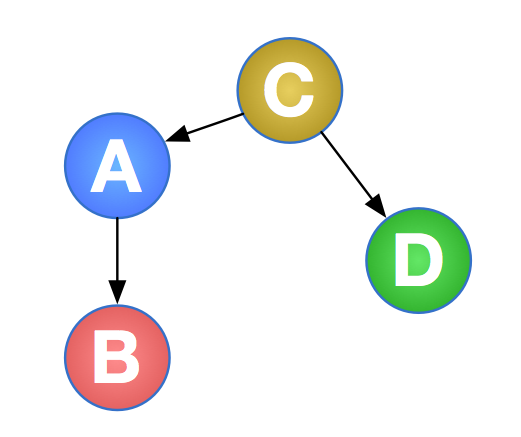
\includegraphics{Resources/ABCD}
	\caption{An example figure of an interaction mapping between arbitrary coloured dots labelled A-D.}
\end{figure}

%\end{multicols}
\section{Modelling}

To apply the formulated model, a \texttt{python} module was developed to numerically solve the outlined system of equations using \texttt{scipy} and \texttt{numpy}. An interactive web-app was developed using \texttt{streamlit} to ease model exploration. 

\large THE APP IS AVAILABLE WHERE??....


%\begin{multicols}{3}
\section{Discussion}

\lipsum[9]

\subsection{Subsub2}
\lipsum[100]
This is a \footnote{Something of a footnote here...} Text of note.

\lipsum[5]

\begin{Acknowledgements}
I would like to thank myself for making this awesome layout. And Felix for having introduced me to LaTeX in the first place :-).	
\end{Acknowledgements}

%\end{multicols}
\section{Supplementary Data}
\setcounter{section}{\thesection+1}
\printbibliography


\end{document}